\section{Processi organizzativi}

\subsection{Gestione di processo}

\subsubsection{Scopo}
Secondo lo standard ISO-12207 la gestione di processo contiene le attività e i compiti generici che vengono impiegati per gestire i vari processi.\\
Il Responsabile di progetto è responsabile della gestione di: del prodotto, del progetto, e delle attività o processi ad esso applicabili.
\subsubsection{Aspettative}
Le aspettative per questo processo sono:
\begin{itemize}
    \item coordinare e semplificare la comunicazione tra i membri del team, assegnando alle singole componenti ruoli e compiti da svolgere;
    \item avere il controllo sul progetto, monitorando il lavoro del team ed in che stato sono i compiti da svolgere;
    \item avere una buona pianificazione delle attività da seguire.
\end{itemize}

\subsubsection{Descrizione}
Questo processo consiste nelle seguenti attività:
\begin{itemize}
    \item iniziazione e definizione dello scopo;
    \item inizializzazione dei processi;
    \item pianificazione di risorse, tempi e costi;
    \item assegnazione dei ruoli e dei compiti;
    \item esecuzione e controllo;
    \item revisione e valutazione.
\end{itemize}

\subsubsection{Coordinamento}
L'attività di coordinamento consente di gestire la comunicazione sia interna che esterna, e le riunioni. Ciò viene fatto attraverso comportamenti precisi che ogni membro del gruppo deve avere per l'intera durata del processo.

\paragraph{Comunicazioni}
Oltre che la comunicazione all'interno del gruppo (Comunicazione interna), durante lo sviluppo del progetto il team si troverà a comunicare con diversi attori esterni:
\begin{itemize}
    \item \textbf{proponente}: RedBabel;
    \item \textbf{committenti}: Prof. Tullio Vardanega e Prof. Riccardo Cardin;
    \item \textbf{competitor}: verranno valutati dopo la Revisione dei requisiti.
\end{itemize}

\subparagraph{Comunicazione interna}
Viene utilizzata come piattaforma principale Slack per comunicazioni che abbiano lo scopo di coordinamento o decisionale, mentre per comunicazioni meno importanti e più informali può essere utilizzato un gruppo Telegram.
Le discussioni su Slack dovranno essere svolte all'interno del canale appropriato, e qual ora si ritenga necessario crearne uno nuovo va fatta segnalazione al Responsabile di progetto che provvederà a valutarne la creazione.\\
I canali di discussione sono organizzati nel seguente modo:
\begin{itemize}
    \item un canale per ogni documento dove si discute del contenuto dello stesso;
    \item \textbf{\#glossario}: per discutere ciò da aggiungere al glossario e delle relative definizioni;
    \item \textbf{\#scadenze}: per scrivere le scadenze future;
    \item \textbf{\#proponente}: discutere di argomenti che probabilmente avranno un coinvolgimento del proponente per porgli delle domande;
    \item \textbf{\#varie}: canale per avere comunicazioni di carattere generale.
\end{itemize}
Un'altra piattaforma di cui ci si avvale è Discord, la quale attraverso le chat vocali può essere utilizzata per svolgere dei compiti o attività con altri membri. In caso di problemi è possibile utilizzare Zoom, in quanto applicazione utilizzata e conosciuta da tutto il team.

\subparagraph{Comunicazione esterna}
Il gruppo è provvisto di un indirizzo email che verrà utilizzato per comunicazioni esterne, il particolare per comunicazioni verso i committenti. Il controllo e l'utilizzo della casella di posta elettronica è vincolato al solo Responsabile di progetto, il quale ha anche il dovere di informare gli altri membri alla ricezione di eventuali comunicazioni.
I membri del team sono altresì presenti all'interno dello Slack del proponente. I canali in questo caso sono due:
\begin{itemize}
    \item \textbf{\#swe-2020\_2021}: canale di discussione in cui sono presenti anche gli altri gruppi che svolgono lo stesso capitolato
    \item \textbf{\#swexception}: canale del gruppo in cui poter fare domande al proponente.
\end{itemize}

\paragraph{Riunioni}
Per ogni riunione, sia essa interna od esterna, verrà nominata una persona incaricata di prendere appunti e far rispettare l'ordine del giorno. Al termine della riunione avrà anche il compito di redarre il verbale e farlo avere agli altri membri entro breve tempo.

\subparagraph{Riunioni interne}
È consentita la partecipazione ai soli membri del team, e per essere svolta deve essere presente più del $50\%$ delle componenti del gruppo. Vengono svolte su una stanza Zoom creata appositamente, o in alternativa in caso di problemi su Discord in una chat vocale dedicata.

\subparagraph{Riunioni esterne}
Sono svolte con i proponenti o committenti, e si terranno su GMeet per riunioni con i proponenti e su Zoom per quelle con i committenti. Il link per il collegamento verrà comunicato dai soggetti esterni nel momento in cui si pianifica un incontro con essi.

\subsubsection{Pianificazione}
Questa sezione ha lo scopo di definire come si intende pianificare il lavoro che c'è da svolgere, come vengono assegnati i compiti tra i membri del gruppo, e in cosa consistono i singoli ruoli.

\paragraph{Ruoli di progetto}
I ruoli, cioè le rispettive figure aziendali che ogni membro del gruppo deve coprire, saranno assegnati in modo tale che ognuno di essi sia stato ricoperto per un numero simile di ore da ogni componente del gruppo. Nel fare ciò bisognerà evitare conflitti di interesse, cioè un componente non potrà verificare un prodotto da lui stesso realizzato. \\
I ruoli che saranno ricoperti nel corso del progetto sono:
\begin{itemize}
    \item Responsabile di progetto;
    \item Amministratore di progetto;
    \item Analista;
    \item Progettista;
    \item Programmatore;
    \item Verificatore.
\end{itemize}

\subparagraph{Responsabile di progetto}
Il Responsabile di progetto è un ruolo fondamentale che deve essere ricoperto per l'intera durata del progetto. Il suo compito principale è coordinare il team e rappresentarlo verso l'esterno. \\
In particolare questo ruolo comporta:
\begin{itemize}
    \item responsabilità di scelte e approvazioni;
    \item responsabilità sulla pianificazione delle attività rispettando le scadenze;
    \item coordinare i membri del gruppo e i compiti da svolgere;
    \item controllare, coordinare e relazionarsi verso soggetti esterni;
    \item avere conoscenze e capacità per saper valutare rischi, scelte, alternative.
\end{itemize}

\subparagraph{Amministratore di progetto}
L'Amministratore di progetto è la figura che ha il controllo sull'ambiente di lavoro, pertanto il suo ruolo comporta i seguenti punti:
\begin{itemize}
    \item amministrare le infrastrutture e servizi di supporto;
    \item risolvere problemi legati alla gestione dei processi;
    \item salvaguardare la documentazione di progetto, controllando che venga verificata e corretta;
    \item controllare il versionamento e le configurazioni dei prodotti;
    \item individuare strumenti che portino ad una maggiore automazione dei processi.
\end{itemize}

\subparagraph{Analista}
L'Analista si occupa di studiare a pieno il problema comprendendone tutte le caratteristiche. Questo ruolo è fondamentale nella fase iniziale, in particolare nella stesura dell'Analisi dei requisiti, in quanto errori o mancanze in questa fase potrebbe compromettere il risultato del progetto.\\
Si deve occupare di:
\begin{itemize}
    \item studiare il dominio del problema;
    \item analizzare e definire le richieste e quindi anche i requisiti del proponente, anche ciò che non è detto esplicitamente;
    \item analizzare dove poi verrà applicato il prodotto finito, quindi i relativi casi d'uso;
    \item redigere lo Studio di fattibilità e l'Analisi dei requisiti.
\end{itemize}

\subparagraph{Progettista}
Il Progettista per prima cosa deve sviluppare una soluzione al problema precedentemente analizzato dagli analisti, soddisfandone i requisiti individuati.\\
Chi ricopre questo ruolo deve:
\begin{itemize}
    \item creare un'architettura che sia coerente e consistente nelle sue parti;
    \item scegliere una soluzione che sia realizzabile nei costi stabiliti;
    \item cercare di limitare le dipendenze tra le varie componenti;
    \item far si che il prodotto possa essere nelle sue parti riusabile.
\end{itemize}

\subparagraph{Programmatore}
Il Programmatore è colui che si occupa della codifica, cioè deve implementare l'architettura che gli viene data dal Progettista.\\
In particolare questo ruolo consiste nel:
\begin{itemize}
    \item codificare ciò che viene passato dal Progettista, documentando e versionando il tutto per agevolare la manutenzione;
    \item scrivere il Manuale utente del codice del prodotto.
\end{itemize}

\subparagraph{Verificatore}
Il Verificatore è un ruolo presente per l'intera durata del progetto e si occupa di controllare che le attività vengano svolte nel rispetto delle norme e della qualità aspettata.\\
I suoi compiti sono:
\begin{itemize}
    \item controllare che le attività si siano concluse senza la presenza di errori;
    \item incaricare chi di dovere di correggere eventuali problemi riscontrati durante lo svolgimento di un'attività;
    \item redigere la parte di retrospettiva del Piano di qualifica.
\end{itemize}

\paragraph{Assegnazione delle attività}
Una volta che sono state individuate le attività da svolgere esse verranno aggiunte dal Responsabile di progetto al servizio di issue-tracking-sistem proposto da GitHub.
Attraverso tale sistema il responsabile di progetto può in qualunque momento valutare come il gruppo sta procedendo ad effettuare il lavoro richiesto.\\
I compiti (Issue) vengono tipicamente autoassegnati dai singoli componenti del gruppo. Si lascia al responsabile di progetto la facoltà di assegnare esplicitamente delle attività a una o più persone nel caso riscontri almeno uno dei seguenti punti:
\begin{itemize}
    \item ci siano issue che sono in attesa di essere svolte da troppo tempo;
    \item ci sia una certa urgenza nel svolgere alcune attività;
    \item ritiene più adatto allo svolgimento di un compito specifici componenti del gruppo.
\end{itemize}
Per evitare la situazione di interverto del responsabile di progetto i singoli membri del team sono portati a scegliere le issue da svolgere tenendo in considerazione di:
\begin{itemize}
    \item dare priorità alle issue con scadenza più vicina;
    \item dare priorità alle issue più vecchie ed ancora non svolte;
    \item scegliere delle issue il cui lavoro sia in un contesto conosciuto, per esempio se ci si ha già lavorato nel corso delle ultime attività svolte.
\end{itemize}
I componenti del gruppo, una volta che un compito è a loro assegnato, sono tenuti a portarlo a termine entro la data prefissata, e sono responsabili della chiusura della relativa issue.

\paragraph{Ciclo di vita di un'attività}
\begin{center}
    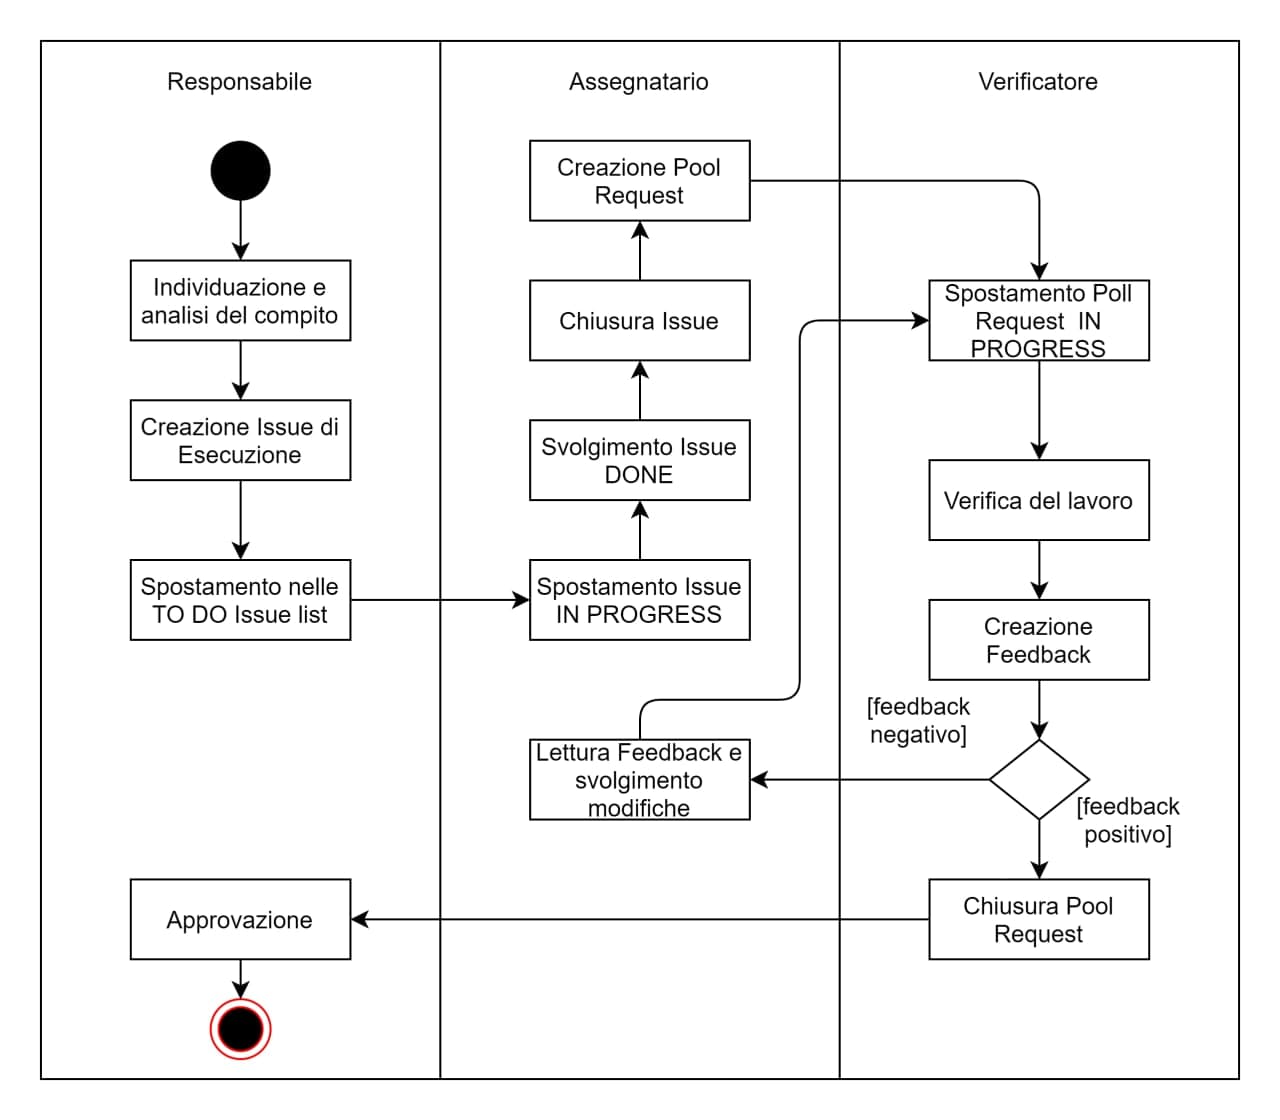
\includegraphics[scale=1.6]{res/images/ciclo_di_vita_ticket.jpg}
\end{center}
Il ciclo di vita di una singola attività interessa tre figure:
\begin{itemize}
    \item \textbf{responsabile di progetto}: individua i compiti da svolgere, e una volta che essi vengono svolti e verificati li approva;
    \item \textbf{assegnatario}: si prende in carico una attività (o gliene viene incaricata una dal responsabile), la svolge, ed a lavoro terminato crea una pool request incaricando un soggetto per effettuare la verifica.
    \item \textbf{verificatore}: controlla e verifica il lavoro che è stato svolto, dopo di che creerà un feedback all'interno della pool request con le correzioni da svolgere nel caso ce ne siano, altrimenti segnalerà completata la pool request e il lavoro in essa contenuto.
\end{itemize}

Le fasi del ciclo di vità di un'attività sono qui spiegate nel dettaglio:
\begin{itemize}
    \item \textbf{individuazione del compito}: dopo aver rilevato nuove necessità, il responsabile di progetto le identifica come richieste da soddisfare creando appunto un nuovo compito. Ne valuta la complessità ed eventualmente lo suddivide in compiti più piccoli. Per ognuno determina una data di scadenza e se lo ritiene necessario può individuare uno o più assegnatari;
    \item \textbf{creazione issue di esecuzione}: il responsabile crea una issue su GitHub identificandola con un titolo esplicativo. Provvede ad inserire nella descrizione la data di scadenza precedentemente stabilità, ed eventualmente una breve descrizione del lavoro da svolgere;
    \item \textbf{spostamento issue in "TO-DO"}: il responsabile sposta la issue nella colonna "TO-DO" all'interno della board di progetto, così da identificarla come da svolgere;
    \item \textbf{spostamento issue in "IN PROGRESS"}: una volta che un assegnatario decide di iniziare il lavoro dopo essersi autoassegnato la issue, o dopo che il responsabile di progetto gli abbia incaricato l'attività, provvederà a spostarla nella colonna "IN PROGRESS";
    \item \textbf{spostamento issue in "DONE"}: terminato il lavoro l'assegnatario provvederà a spostare la issue in "DONE" ed a chiudere la issue;
    \item \textbf{creazione pool request}: l'assegnatario a questo punto dovrà creare una pool request dal ramo contenente il lavoro svolto al ramo di riferimento. Dovrà poi indicare nel campo "Reviewer" un componente incaricato della verifica ed inserire la lable "da revisionare". Può aggiungere alla pool request una descrizione contenente dei commenti sul lavoro svolto se ritiene che ciò possa essere utile al controllo da parte del verificatore. Conclude inserendo la pool request all'interno della sezione "TO-DO" della board di progetto;
    \item \textbf{spostamento pool request in "IN PROGRESS"}: il verificatore quando inizia il lavoro di verifica sposta la pool request in "IN PROGRESS";
    \item \textbf{creazione feedback di verifica}: terminata la verifica il verificatore scrive un feedback del lavoro sottopostogli, e richiede delle modifiche nel caso riscontri delle correzioni da fare. In questo caso assegna la pool request al componente del gruppo che la creata, e modifica la label in "da correggere";
    \item \textbf{svolgimento modifiche}: l'assegnatario dopo aver ricevuto dal verificatore un feedback sulle cose da sistemare provvederà a svolgerle. Una volta terminate le correzioni richiederà un'ulteriore verifica attraverso il tasto "re-reviews" e modificherà la lable in "da revisionare";
    \item \textbf{spostamento pool request in "DONE"}: se il verificatore non riscontra correzioni da fare, o quelle effettuate sono sodisfacenti, sposta la pool request in "DONE";
    \item \textbf{approvazione del lavoro}: il responsabile di progetto dopo aver esaminato il lavoro lo approva, e può effettuare il merge con il ramo interesasto.
\end{itemize}
\paragraph{Metriche di processo}

\subparagraph{Budgeted Cost of Work Scheduled - BCWS}
Rappresenta il costo pianificato in euro per realizzare le attività di progetto alla data corrente.

\subparagraph{Actual Cost of Work Performed - ACWP}
Rappresenta il costo effettivamente sostenuto in euro alla data corrente.

\subparagraph{Budgeted Cost of Work Performed - BCWP}
Rappresenta il valore in euro delle attività realizzate alla data corrente.

\subparagraph{Cost Variance - CV}
Indica se il valore realmente maturato è maggiore, uguale o minore rispetto al costo effettivo.
\begin{itemize}
    \item \textbf{Formula}: $CV = BCWP - ACWP$
    \item \textbf{Risultato}: se $CV > 0$ significa che il progetto produce con maggior efficienza (minor costo) rispetto a quanto pianificato, viceversa se negativo.
\end{itemize}

\subparagraph{Schedule Variance - SV}
Indica se si è in linea, in anticipo o in ritardo rispetto alla schedulazione delle attività di progetto pianificate nella baseline.
\begin{itemize}
    \item \textbf{Formula}: $SV = BCWP - BCWS$
    \item \textbf{Risultato}: se $SV > 0$ significa che il progetto sta producendo con maggior velocità a quanto pianificato, viceversa se negativo.
\end{itemize}